\documentclass[draftclsnofoot,onecolumn,letterpaper,10pt]{IEEEtran}

\usepackage{geometry}
\geometry{textheight=9.5in, textwidth=7in}

\usepackage{float}
\usepackage{graphicx}
\usepackage{algorithm2e}
\usepackage{pgfgantt}
\usepackage{booktabs}
\graphicspath{ {images/} }

\newcommand{\subparagraph}{}
\usepackage{titlesec}

\begin{document}
\begin{center}
	{\huge\textbf{Senior Software Engineering Design Group 7}}
	\vspace{1cm}

	{\Huge\textbf{brew.ai Progress Report -- Spring Term}}

	\vspace{2cm}
	\textbf{Connor Yates}\\yatesco@oregonstate.edu

	\textbf{Aravind Parasurama}\\parasura@oregonstate.edu

	\textbf{Cody Holliday}\\hollidac@oregonstate.edu

	\vspace{2cm}
	{\Large CS 463, Spring 2017}
	\vspace{1cm}
\end{center}

\begin{abstract}

\end{abstract}

\newpage
\tableofcontents
\newpage

\section{Purposes and Goals}
\subsection{Project Purpose}
Brew.ai is a hardware and software solution for automated brewing of mead or beer.
Currently, home brewing requires a lot of time, knowledge, and patience.
As such, it is not accessible to amateurs, and brew.ai seeks to solve this problem.
From amateurs to professional brewers, we want brew.ai to be useful by automating the brewing process and helping brewers make better tasting products.

\subsection{Project Goals}
At the end of the project, we look to produce a physical device that contains the necessary electronics and software to control the brewing process.
The brew.ai device itself is a bucket lid that will fit over a brewing device and have various modules incorporated in it.
The lid device will monitor and control temperature, send and receive commands/data to and from the Android application, and monitor fermentation status.
From the perspective of a user, setup will be essentially plug-and-play.
No technical knowledge is needed beyond knowing how to pair a Bluetooth device an Android device, open an app, and put ingredients into a bucket.
brew.ai also will improve on its recipe over time by leveraging the power of reinforcement learning and the users own feedback on the product it creates.
A main goal of this project is creating a product with the ability to learn from each batch, and improve its performance.

\section{Current Project Status}

\subsection{Hardware\\{\em\textbf{Aravind Parasurama}}}
\subsubsection{Overview}

\subsubsection{Current Status}
\begin{figure}
\label{fig:hw1}
\caption{The first protoype of the brewing hardware with stirring element detached.}
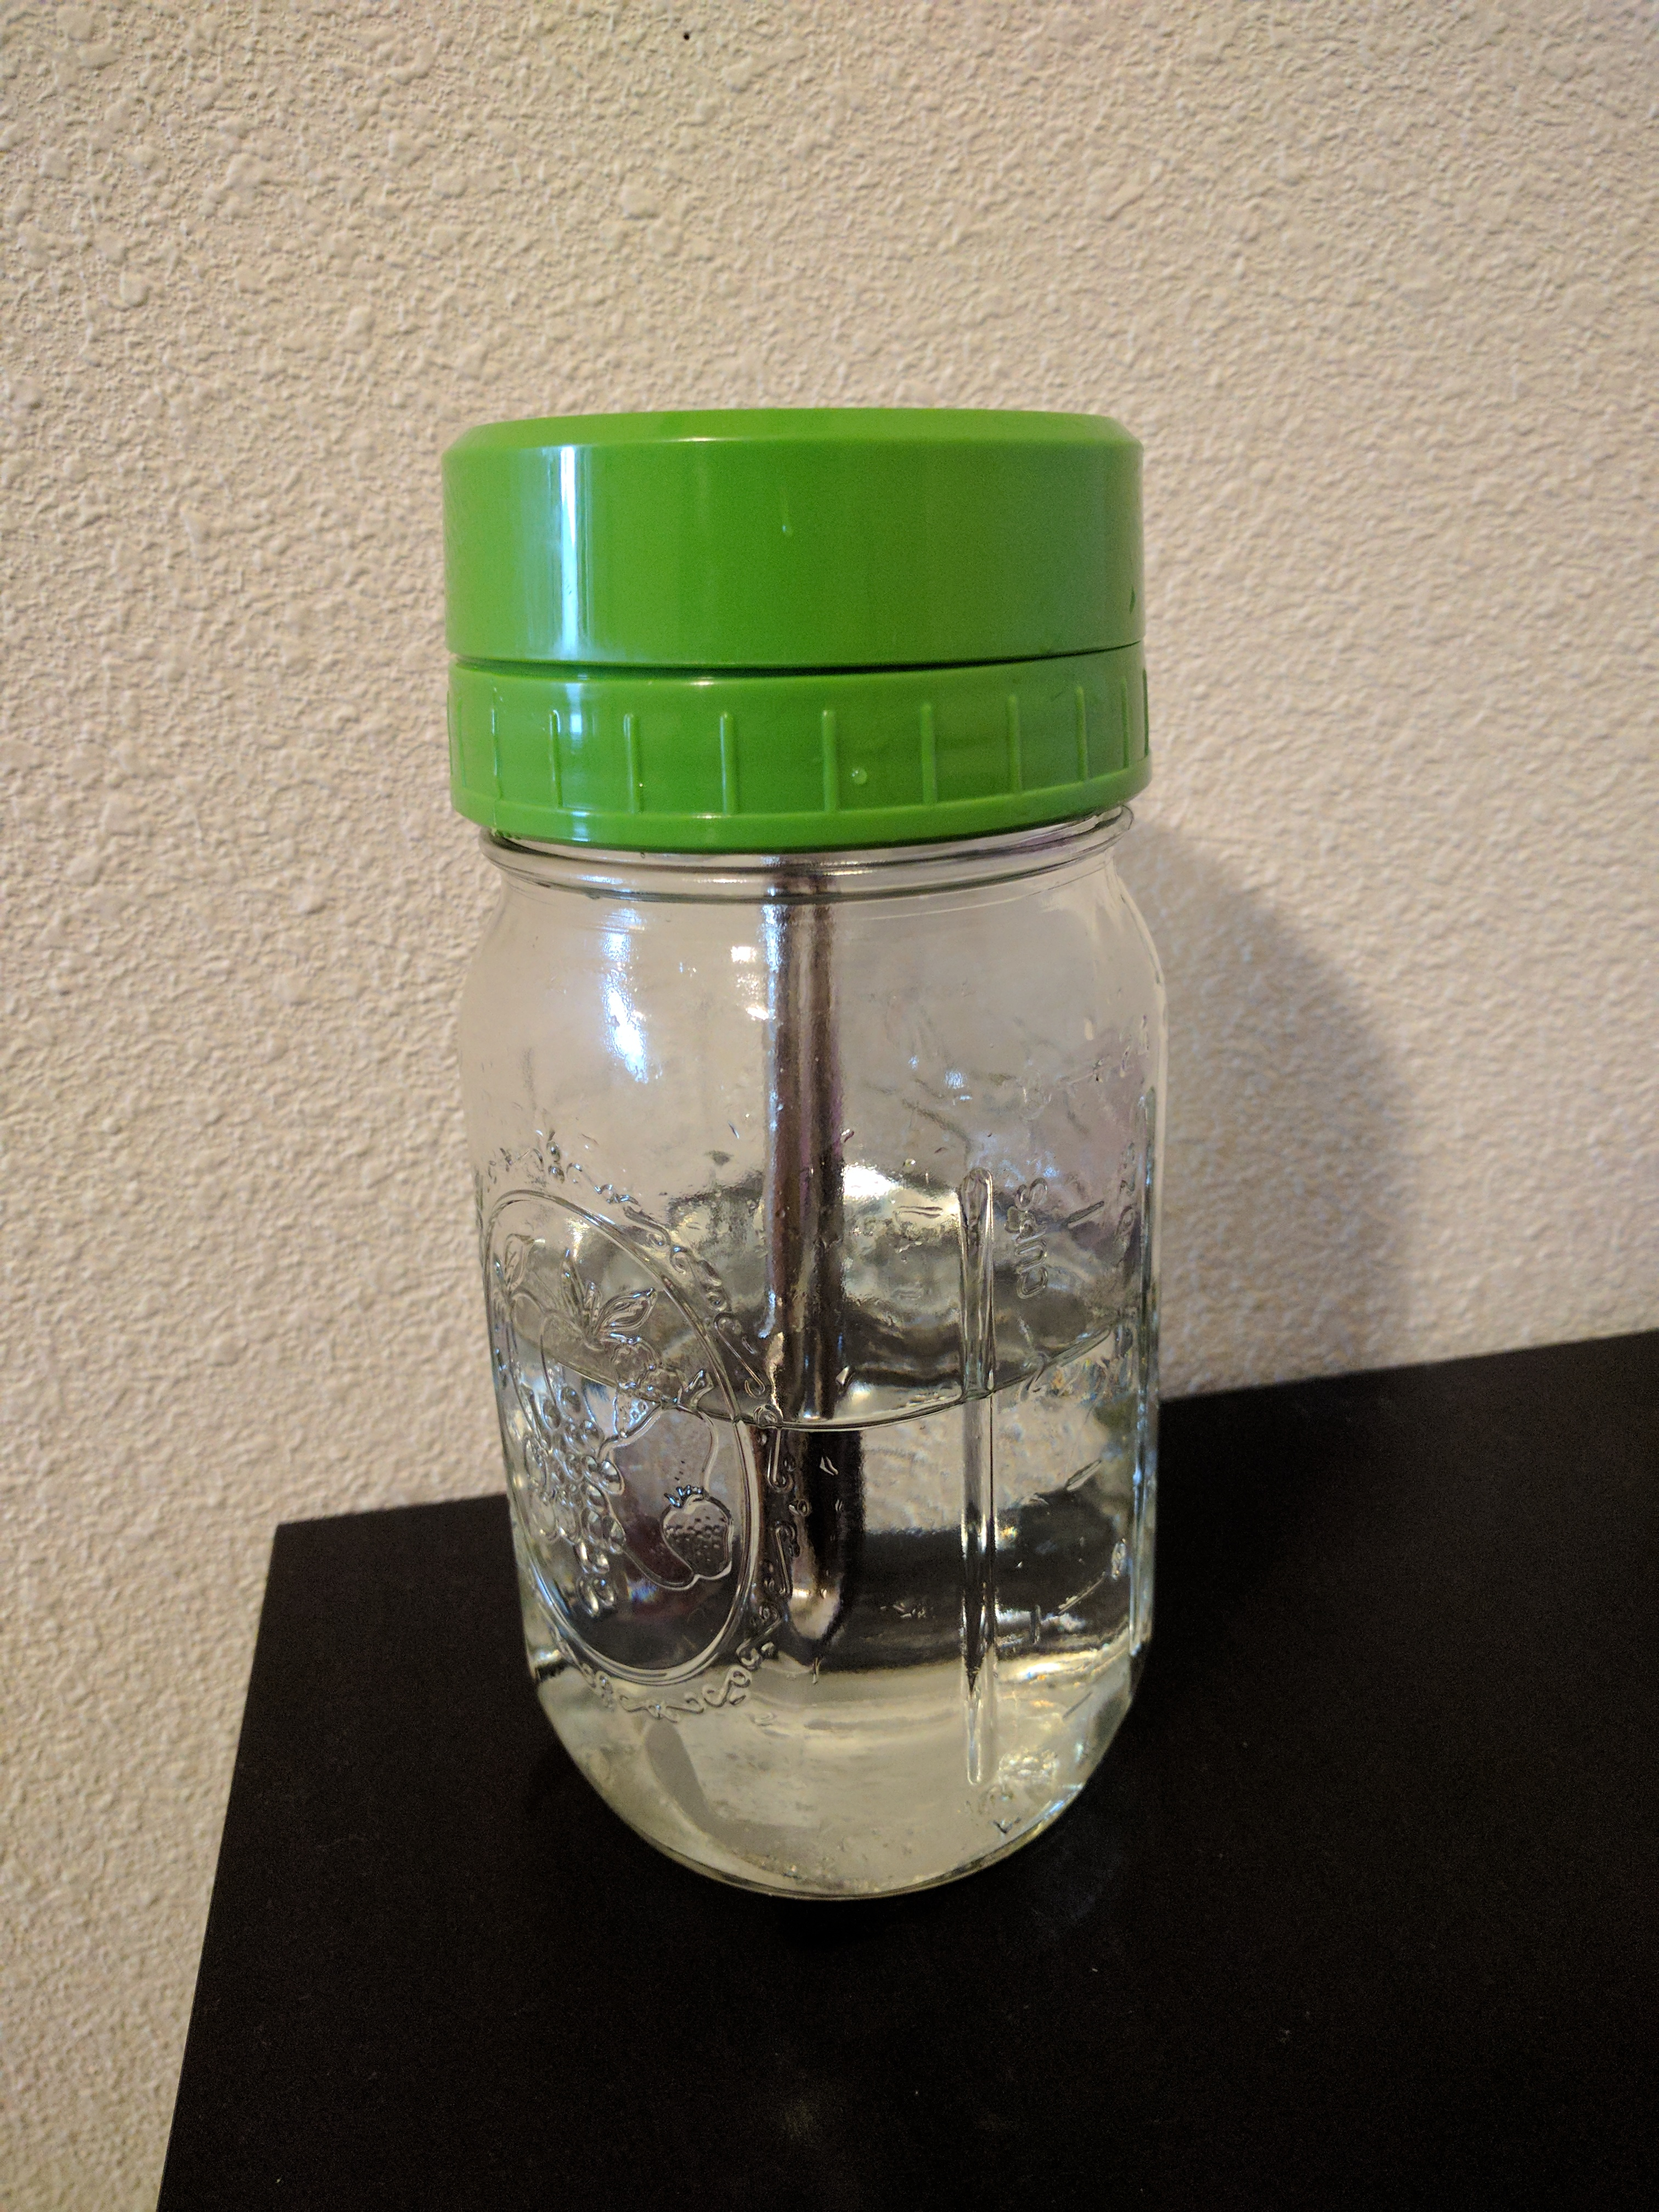
\includegraphics[width=\linewidth]{hw1.eps}
\end{figure}

\subsubsection{Tasks Left}

\subsubsection{Roadblocks}

\subsection{Android Interface\\{\em\textbf{Cody Holliday}}}


\subsubsection{Work Done and Roadblocks}

\newpage
\vfill

\begin{figure}
\label{fig:layout}
\caption{Here is the layout of the app currently.}
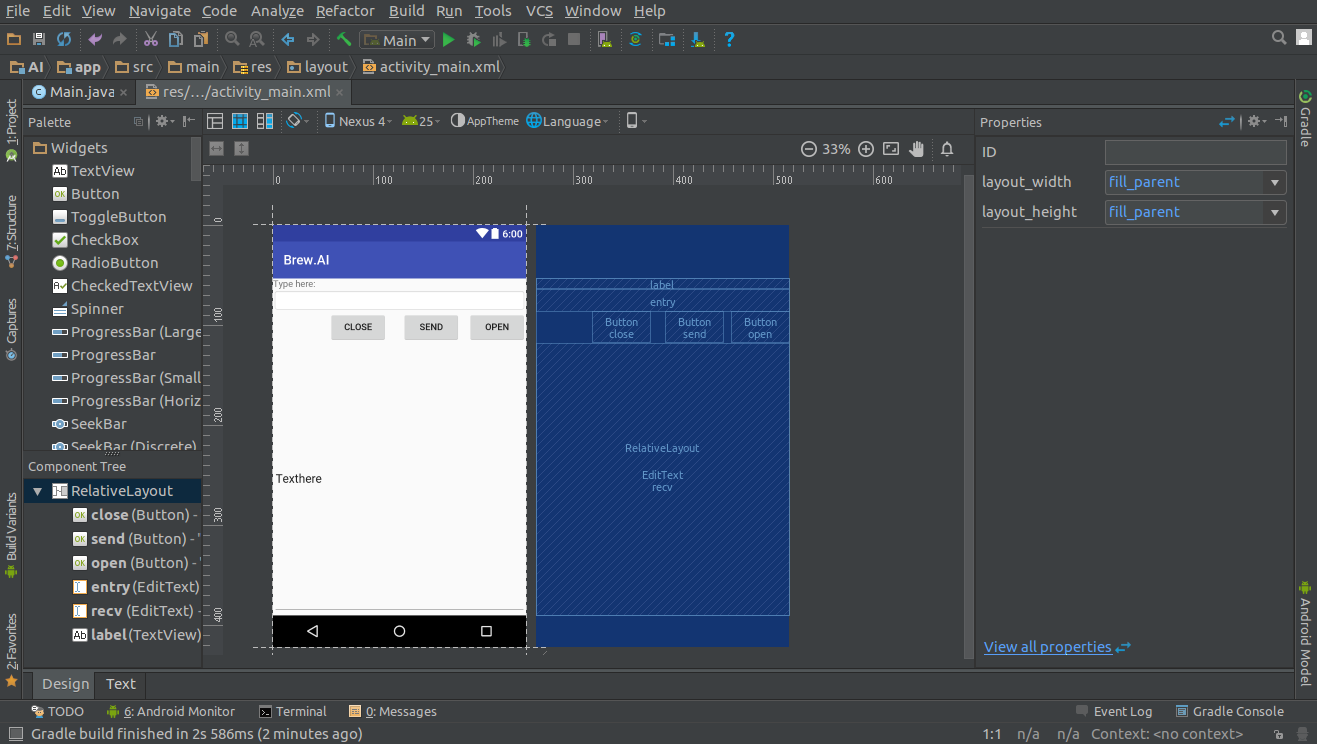
\includegraphics[scale=0.4]{android-layout.eps}
\end{figure}


\begin{figure}
\label{fig:code}
\caption{This is some of the code for button functionality.}
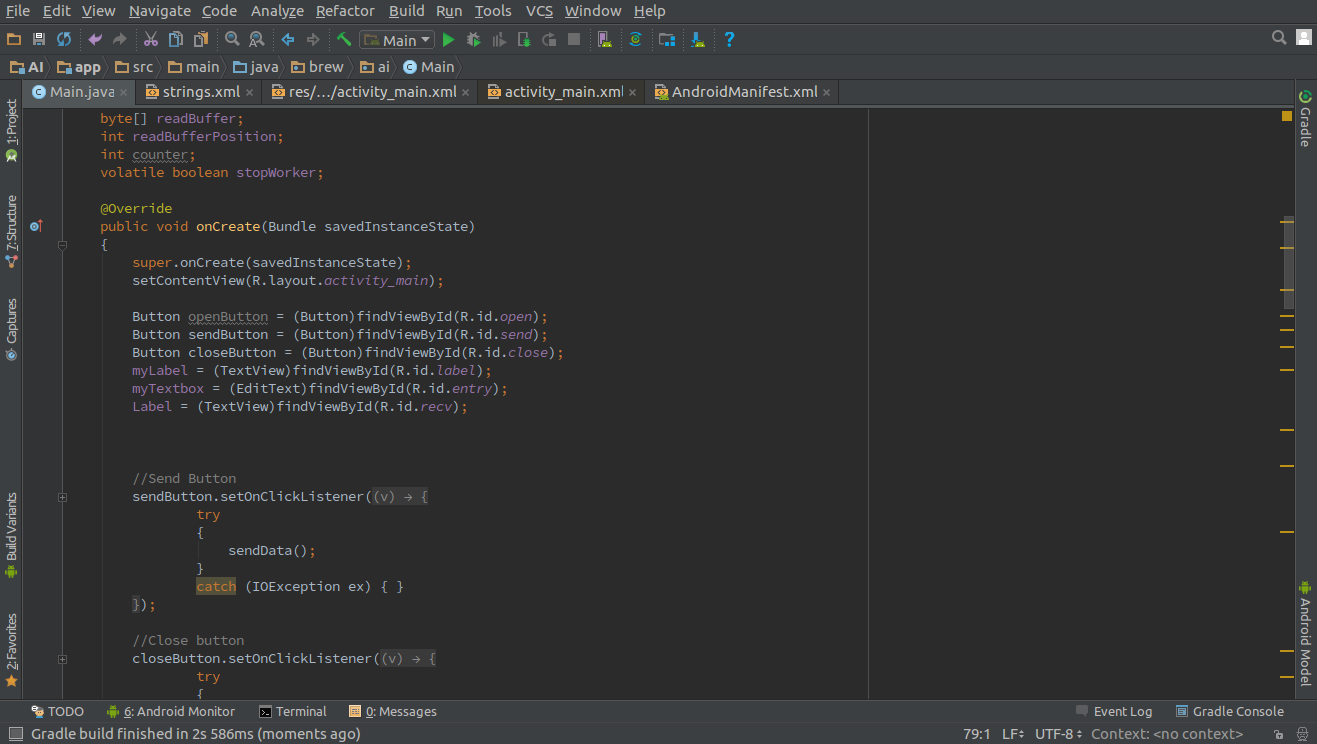
\includegraphics[scale=0.4]{android-code.eps}
\end{figure}


\begin{figure}
\label{fig:python}
\caption{This is the python script written to transmit and receive information.}
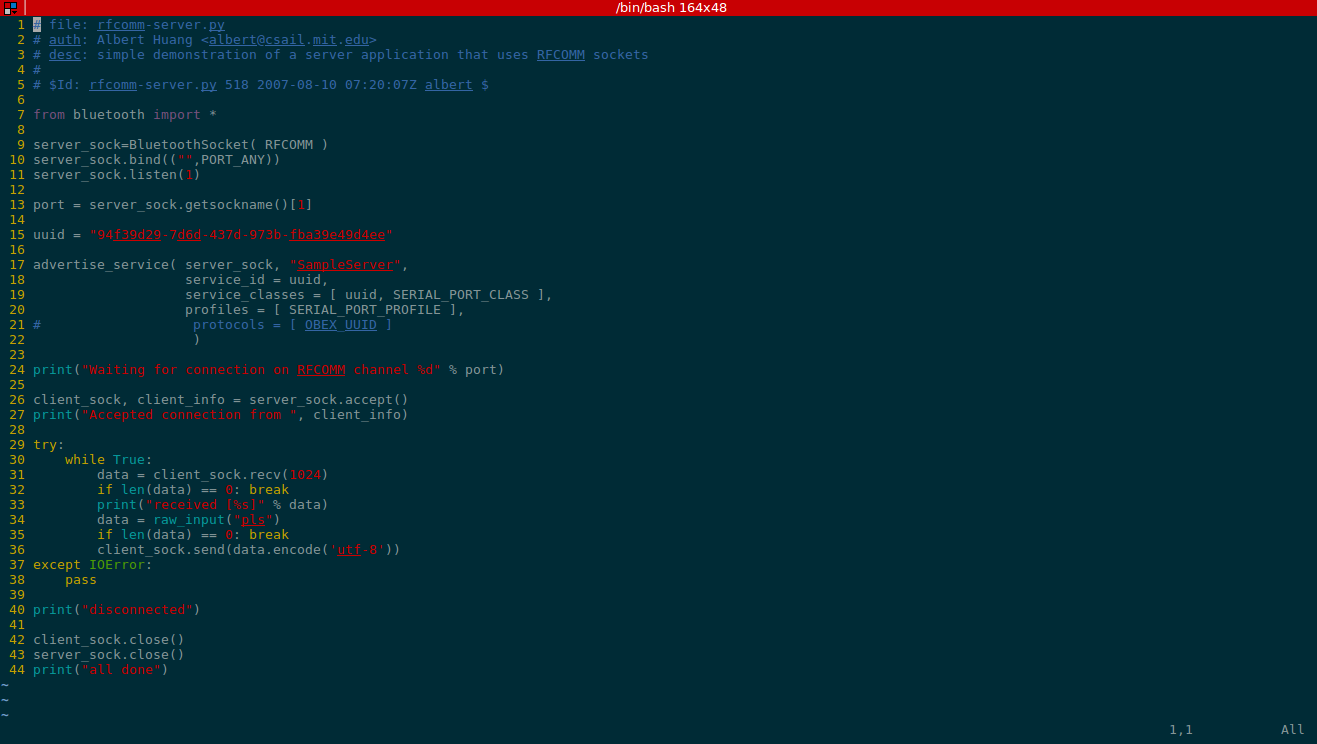
\includegraphics[scale=0.4]{python-server.eps}
\end{figure}

\vfill
\clearpage
\subsubsection{Work Left Undone}

\subsubsection{App Design}


\subsection{Artificial Intelligence\\{\em\textbf{Connor Yates}}}
\subsubsection{AI Review and Purpose}


\subsubsection{AI Progress}

\subsubsection{Simple Simulator}

\subsubsection{Roadblocks and Solutions}


\section{Summary}

\end{document}
